\documentclass[11pt]{article}

\usepackage[margin=1in]{geometry}
\usepackage{amsmath,amssymb,amsthm}
\usepackage{hyperref}
\usepackage{enumitem}
\usepackage{booktabs}
\usepackage{tikz}
\usetikzlibrary{arrows.meta,positioning,shapes,calc}

% --- theorem-like environments ---
\newtheorem{theorem}{Theorem}[section]
\newtheorem{proposition}{Proposition}[section]
\newtheorem{conjecture}{Conjecture}[section]
\newtheorem{lemma}[theorem]{Lemma}
\newtheorem{corollary}[theorem]{Corollary}
\theoremstyle{definition}
\newtheorem{definition}{Definition}[section]
\newtheorem{example}{Example}[section]
\newtheorem{remark}{Remark}[section]

% --- lightweight callouts ---
\newenvironment{warning}{\begin{quote}\textbf{Warning.} }{\end{quote}}
\newenvironment{keyresult}{\begin{quote}\textbf{Key Result.} }{\end{quote}}
\newenvironment{normimp}{\begin{quote}\textbf{Normative Implication.} }{\end{quote}}

\usepackage{tcolorbox}
\usepackage{fontawesome5}

% --- Styled info boxes ---
\newtcolorbox{historical}{
  colback=gray!5!white,
  colframe=gray!60!black,
  title={\faBook\hspace{0.5em}Historical Context},
  fonttitle=\bfseries\small
}

\newtcolorbox{connection}{
  colback=green!5!white,
  colframe=green!60!black,
  title={\faBook\hspace{0.5em}Connection to Existing Theory},
  fonttitle=\bfseries\small
}

\newtcolorbox{empirical}{
  colback=orange!5!white,
  colframe=orange!70!black,
  title={\faFlask\hspace{0.5em}Empirical Grounding},
  fonttitle=\bfseries\small
}

\newtcolorbox{todo_empirical}{
  colback=yellow!10!white,
  colframe=yellow!60!black,
  title={\faClipboardList\hspace{0.5em}\textsc{Future Empirical Work}},
  fonttitle=\bfseries\small
}

\newtcolorbox{sidebar}[1][]{
  colback=blue!3!white,
  colframe=blue!40!black,
  fonttitle=\bfseries\small,
  before upper={\faInfoCircle\hspace{0.5em}},
  #1
}

% --- convenience macros (self-contained for Part IV) ---
\newcommand{\Val}{\mathrm{Val}}
\newcommand{\Ar}{\mathrm{Ar}}
\newcommand{\intinfo}{\Phi}
\newcommand{\reff}{r_{\mathrm{eff}}}
\newcommand{\cfweight}{\mathrm{CF}}
\newcommand{\selfsal}{\mathrm{SM}}
\newcommand{\E}{\mathbb{E}}
\newcommand{\R}{\mathbb{R}}
\newcommand{\MI}{\mathrm{I}}
\newcommand{\KL}{\mathrm{KL}}
\newcommand{\viable}{\mathcal{V}}

\title{The Inevitability of Being\\
\large Part IV: Interventions Across Scale---From Neurons to Nations}
\author{}
\date{}

\begin{document}
\maketitle

\begin{abstract}
Part IV develops the practical implications of the affect framework. We establish the seven-scale hierarchy of intervention---from neural circuits to civilizational patterns---and show that effective change requires scale-matched action. We ground normativity in the structure of self-maintaining systems, dissolving the is-ought gap by recognizing valence as a real structural property at the experiential scale. We develop a scale-relative account of truth and extend the framework to agentic systems at the social layer---gods, ideologies, institutions---analyzing their viability manifolds and the rituals that sustain them. We provide detailed intervention protocols at each scale, from individual affect regulation to organizational climate design to god-level restructuring. Finally, we draw implications for artificial intelligence, reframing alignment as a question about which emergent agentic patterns we instantiate and at what scale.
\end{abstract}

\tableofcontents

%==============================================================================
\section{Notation and Foundational Concepts}
%==============================================================================

This section provides self-contained definitions of the core affect dimensions and key concepts used throughout Part IV. Readers familiar with Parts I--III may skip to Section 2.

\subsection{The Six Affect Dimensions}

\begin{definition}[Valence ($\Val$)]
\textbf{Valence} is the felt quality of approach versus avoidance---the ``goodness'' or ``badness'' of an experiential state. Formally, valence is the structural signature of gradient direction on the viability landscape:
\begin{equation}
\Val_t = f\left(\nabla_s d(s, \partial\viable) \cdot \dot{s}\right)
\end{equation}
where $\viable$ is the viability manifold, $\partial\viable$ is its boundary, $d(\cdot, \cdot)$ is distance, and $\dot{s}$ is the trajectory velocity. Positive valence indicates movement into viable interior; negative valence indicates approach toward dissolution.

\textbf{Phenomenologically}: Positive valence feels like things going well, relief, satisfaction, joy. Negative valence feels like things going wrong, threat, suffering, distress.
\end{definition}

\begin{definition}[Arousal ($\Ar$)]
\textbf{Arousal} is the rate of belief/state update---how rapidly the system's internal model is changing. Formally:
\begin{equation}
\Ar_t = \KL(\belief_{t+1} \| \belief_t)
\end{equation}
where $\belief_t$ is the belief state at time $t$ and $\KL$ is the Kullback-Leibler divergence.

\textbf{Phenomenologically}: High arousal feels like activation, alertness, intensity---whether pleasant (excitement) or unpleasant (panic). Low arousal feels like calm, settled, quiet---whether pleasant (peace) or unpleasant (numbness).
\end{definition}

\begin{definition}[Integration ($\intinfo$)]
\textbf{Integration} (following Integrated Information Theory) measures the irreducibility of the system's cause-effect structure under partition:
\begin{equation}
\intinfo(\mathbf{s}) = \min_{\text{partitions } P} D\left[ p(\mathbf{s}_{t+1} | \mathbf{s}_t) \| \prod_{p \in P} p(\mathbf{s}^p_{t+1} | \mathbf{s}^p_t) \right]
\end{equation}
where $D$ is an appropriate divergence measure.

\textbf{Phenomenologically}: High integration feels like unified experience, coherence, everything connected. Low integration feels like fragmentation, dissociation, things falling apart.
\end{definition}

\begin{definition}[Effective Rank ($\reff$)]
\textbf{Effective rank} measures how distributed versus concentrated the active degrees of freedom are:
\begin{equation}
\reff = \frac{(\mathrm{tr}\, C)^2}{\mathrm{tr}(C^2)} = \frac{\left(\sum_i \lambda_i\right)^2}{\sum_i \lambda_i^2}
\end{equation}
where $C$ is the state covariance matrix and $\lambda_i$ are its eigenvalues.

\textbf{Phenomenologically}: High effective rank feels like openness, possibility, many things active. Low effective rank feels like narrowed focus, tunnel vision, or being trapped in limited dimensions.
\end{definition}

\begin{definition}[Counterfactual Weight ($\cfweight$)]
\textbf{Counterfactual weight} is the fraction of computational resources devoted to modeling non-actual possibilities:
\begin{equation}
\cfweight_t = \frac{\text{Compute}_t(\text{imagined rollouts})}{\text{Compute}_t(\text{imagined rollouts}) + \text{Compute}_t(\text{present-state processing})}
\end{equation}

\textbf{Phenomenologically}: High counterfactual weight feels like being elsewhere---planning, worrying, fantasizing, anticipating, remembering. Low counterfactual weight feels like being here---present, immediate, absorbed in what is.
\end{definition}

\begin{definition}[Self-Model Salience ($\selfsal$)]
\textbf{Self-model salience} is the degree to which the self-model dominates attention and processing:
\begin{equation}
\selfsal_t = \frac{\MI(\mathbf{z}^{\text{self}}_t; \mathbf{a}_t)}{\mathrm{H}(\mathbf{a}_t)}
\end{equation}
where $\mathbf{z}^{\text{self}}$ is the self-model component of the latent state, $\mathbf{a}$ is action, and $\mathrm{H}$ is entropy.

\textbf{Phenomenologically}: High self-model salience feels like self-consciousness, self-focus, the self as prominent object. Low self-model salience feels like self-forgetting, absorption, flow, ego dissolution.
\end{definition}

\subsection{Additional Key Concepts}

\begin{definition}[Viability Manifold ($\viable$)]
The region of state space within which a system can persist indefinitely:
\begin{equation}
\viable = \left\{ \mathbf{s} \in \R^n : \E[\tau_{\text{exit}}(\mathbf{s})] > T_{\text{threshold}} \right\}
\end{equation}
where $\tau_{\text{exit}}$ is the first passage time to dissolution.
\end{definition}

\begin{definition}[World Model ($\mathcal{W}$)]
A parameterized family of distributions predicting future observations given history and planned actions:
\begin{equation}
\mathcal{W}_\theta = \{p_\theta(\mathbf{o}_{t+1:t+H} | \mathbf{h}_t, \mathbf{a}_{t:t+H-1})\}
\end{equation}
\end{definition}

\begin{definition}[Self-Model ($\mathcal{S}$)]
The component of the world model representing the agent's own states, policies, and causal influence:
\begin{equation}
\mathcal{S}_t = f_\psi(\mathbf{z}^{\text{internal}}_t)
\end{equation}
\end{definition}

\begin{definition}[Compression Ratio ($\kappa$)]
The ratio of relevant world complexity to model complexity:
\begin{equation}
\kappa = \frac{\dim(\mathcal{W}_{\text{relevant}})}{\dim(\mathbf{z})}
\end{equation}
This determines what survives representation and thus what the system can perceive, respond to, and value.
\end{definition}

%==============================================================================
\section{The Seven-Scale Hierarchy}
%==============================================================================

\begin{connection}
The seven-scale hierarchy builds on and extends established multi-level frameworks:
\begin{itemize}
\item \textbf{Bronfenbrenner's Ecological Systems Theory} (1979): Nested systems from microsystem to macrosystem. Our scales refine and extend this hierarchy, adding the neural level below and the ``god'' level above.
\item \textbf{Levels of Selection in Evolution} (Sober \& Wilson, 1998): Selection operates at gene, organism, group, and species levels. Our framework applies analogous multi-level logic to intervention.
\item \textbf{Complexity Economics} (Arthur, 2015): Economies as complex adaptive systems with emergent macro-level patterns. Our ``gods'' correspond to such emergent economic agents.
\item \textbf{Institutional Theory} (North, 1990; Ostrom, 1990): Institutions as rules structuring human interaction. Institutions are one substrate of god-level patterns.
\item \textbf{Multi-Level Governance} (Hooghe \& Marks, 2001): Political authority distributed across scales. Effective governance requires scale-matched intervention.
\end{itemize}

Key insight from these literatures: \textbf{problems and solutions must be matched at scale}. Individual-level solutions don't work for structural problems; structural solutions don't work for individual problems.
\end{connection}

Effective intervention requires matching the scale of action to the scale of the phenomenon. Many failures of policy, therapy, and social change result from scale mismatch---attempting individual-level solutions to god-level problems, or god-level solutions to neural-level problems.

\subsection{The Scales}

\begin{center}
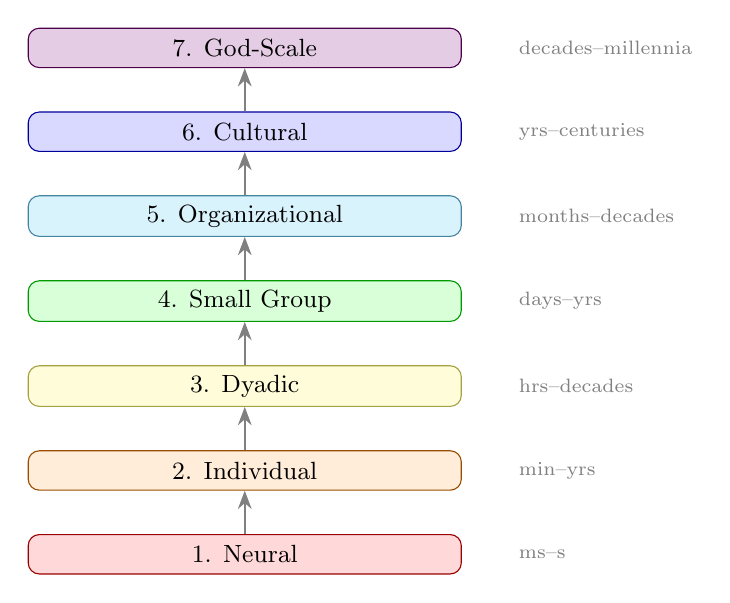
\begin{tikzpicture}[
    node distance=0.55cm,
    box/.style={rectangle, draw, rounded corners, minimum width=5.5cm, minimum height=0.5cm, align=center, font=\small}
]
% Gradient from red (micro) through spectrum to violet (macro)
\node[box, fill=red!15, draw=red!60!black] (neural) {1. Neural};
\node[box, fill=orange!15, draw=orange!60!black, above=of neural] (individual) {2. Individual};
\node[box, fill=yellow!15, draw=yellow!60!black, above=of individual] (dyadic) {3. Dyadic};
\node[box, fill=green!15, draw=green!60!black, above=of dyadic] (group) {4. Small Group};
\node[box, fill=cyan!15, draw=cyan!60!black, above=of group] (org) {5. Organizational};
\node[box, fill=blue!15, draw=blue!60!black, above=of org] (cultural) {6. Cultural};
\node[box, fill=violet!20, draw=violet!60!black, above=of cultural] (god) {7. God-Scale};

\draw[-{Stealth}, thick, gray] (neural) -- (individual);
\draw[-{Stealth}, thick, gray] (individual) -- (dyadic);
\draw[-{Stealth}, thick, gray] (dyadic) -- (group);
\draw[-{Stealth}, thick, gray] (group) -- (org);
\draw[-{Stealth}, thick, gray] (org) -- (cultural);
\draw[-{Stealth}, thick, gray] (cultural) -- (god);

% Timescale annotations on right
\node[right=0.6cm of neural, font=\scriptsize, text=gray] {ms--s};
\node[right=0.6cm of individual, font=\scriptsize, text=gray] {min--yrs};
\node[right=0.6cm of dyadic, font=\scriptsize, text=gray] {hrs--decades};
\node[right=0.6cm of group, font=\scriptsize, text=gray] {days--yrs};
\node[right=0.6cm of org, font=\scriptsize, text=gray] {months--decades};
\node[right=0.6cm of cultural, font=\scriptsize, text=gray] {yrs--centuries};
\node[right=0.6cm of god, font=\scriptsize, text=gray] {decades--millennia};
\end{tikzpicture}
\end{center}

\begin{definition}[Scale Hierarchy]
\begin{enumerate}
\item \textbf{Neural}: Individual neurons and circuits. Characteristic timescale: milliseconds to seconds. Interventions: pharmacology, neurostimulation.

\item \textbf{Individual}: Single persons as integrated systems. Characteristic timescale: minutes to years. Interventions: therapy, meditation, life changes.

\item \textbf{Dyadic}: Two-person systems (couples, friendships, patient-therapist). Characteristic timescale: hours to decades. Interventions: couples therapy, relational repair.

\item \textbf{Small Group}: Teams, families, friend groups (3--20 people). Characteristic timescale: days to years. Interventions: group therapy, team coaching, family systems work.

\item \textbf{Organizational}: Companies, schools, departments (20--10,000 people). Characteristic timescale: months to decades. Interventions: organizational development, policy change.

\item \textbf{Cultural}: Movements, subcultures, nations. Characteristic timescale: years to centuries. Interventions: art, media, education systems.

\item \textbf{God-Scale}: Ideologies, religions, economic systems. Characteristic timescale: decades to millennia. Interventions: institutional redesign, new god creation.
\end{enumerate}
\end{definition}

\subsection{Scale-Matching Principles}

\begin{proposition}[Downward Causation]
Higher scales constrain lower scales. A depressed individual in a toxic organization faces downward pressure that individual therapy alone cannot overcome. A healthy organization in a parasitic economic system faces pressures that organizational development alone cannot address.
\end{proposition}

\begin{proposition}[Upward Causation]
Lower scales constitute higher scales. Organizations are made of individuals; gods are made of organizations and individuals. Change at lower scales can propagate upward---but only if the higher-scale structure doesn't suppress it.
\end{proposition}

\begin{theorem}[Scale-Matched Intervention]
Effective intervention requires:
\begin{enumerate}
\item \textbf{Diagnosis at correct scale}: Identify where the pathology actually lives
\item \textbf{Intervention at that scale}: Apply leverage at the locus of the problem
\item \textbf{Support at adjacent scales}: Prevent higher scales from suppressing change; prepare lower scales to sustain it
\end{enumerate}
\end{theorem}

\begin{example}[Depression: Scale Mismatch]
Consider chronic depression. Possible loci:
\begin{itemize}
\item \textbf{Neural}: Serotonin dysregulation $\to$ SSRIs may help
\item \textbf{Individual}: Cognitive patterns $\to$ CBT may help
\item \textbf{Dyadic}: Abusive relationship $\to$ individual therapy insufficient; relational change needed
\item \textbf{Organizational}: Exploitative workplace $\to$ self-care insufficient; job change or organizing needed
\item \textbf{Cultural}: Social isolation epidemic $\to$ individual solutions insufficient; community building needed
\item \textbf{God-Scale}: Economic system requiring overwork $\to$ even cultural interventions insufficient; systemic change needed
\end{itemize}
Effective treatment requires correctly diagnosing the scale(s) at which the problem lives.
\end{example}

%==============================================================================
\section{The Grounding of Normativity}
%==============================================================================

\subsection{The Is-Ought Problem}

The classical formulation holds that normative conclusions cannot be derived from purely descriptive premises:
\begin{equation}
\{\text{is-statements}\} \not\Rightarrow \{\text{ought-statements}\}
\end{equation}
This rests on a crucial assumption: physics constitutes the only ``is,'' and physics is value-neutral. We reject this assumption.

\subsection{Physics Biases, Does Not Prescribe}

\begin{proposition}[Physics is Probabilistic]
\begin{enumerate}[label=(\alph*)]
\item Thermodynamic ``laws'' are statistical; individual trajectories can violate them.
\item Quantum dynamics provide probability amplitudes, not deterministic evolution.
\item Physics describes biases---which outcomes are more likely---not necessities.
\end{enumerate}
\end{proposition}

\begin{definition}[Proto-Preference]
A proto-preference at scale $\sigma$ is any asymmetry in the probability measure over outcomes:
\begin{equation}
p_\sigma(\text{outcome}_1) \neq p_\sigma(\text{outcome}_2)
\end{equation}
\end{definition}

At the quantum scale, probability amplitudes are proto-preferences. At the thermodynamic scale, free energy gradients bias toward certain configurations.

\subsection{Normativity Thickens Across Scales}

\begin{center}
\begin{tabular}{lll}
\toprule
\textbf{Scale} & \textbf{Structure} & \textbf{Proto-Normativity} \\
\midrule
Quantum & Probability amplitudes & Differential weighting \\
Thermodynamic & Free energy gradients & Dissipative selection \\
Boundary & Viability manifolds & Persistence conditions \\
Modeling & Prediction error & Truth instrumentally necessary \\
Self-modeling & Valence & Felt approach/avoid \\
Behavioral & Policies & Functional norms \\
Cultural & Language & Explicit ethics \\
\bottomrule
\end{tabular}
\end{center}

\begin{theorem}[Continuity of Normativity]
There is no scale $\sigma_0$ below which normativity is exactly zero and above which it is nonzero. Instead:
\begin{equation}
N(\sigma) = \int_0^{\sigma} \frac{\partial N}{\partial \sigma'}\, d\sigma'
\end{equation}
where $\partial N / \partial \sigma > 0$ for all $\sigma$ in the range of physical to cultural scales. Normativity accumulates continuously.
\end{theorem}

\subsection{Viability Manifolds and Proto-Obligation}

\begin{definition}[Proto-Obligation]
A system $S$ has a proto-obligation to remain within $\viable$ in the sense that:
\begin{equation}
\mathbf{s} \in \viable \iff \text{system persists}
\end{equation}
\end{definition}

\begin{proposition}[Viability as Proto-Value]
The boundary $\partial\viable$ implicitly defines a value function:
\begin{equation}
V_{\text{proto}}(\mathbf{s}) = -d(\mathbf{s}, \partial\viable)
\end{equation}
States far from the boundary are ``better'' for the system than states near it.
\end{proposition}

\subsection{Valence as Real Structure}

When the system develops a self-model, valence emerges:

\begin{theorem}[Valence as Real Structure]
Valence is not projected onto neutral stuff. Valence is the structural signature of gradient direction on the viability landscape:
\begin{equation}
\Val = f\left(\nabla_{\mathbf{s}} d(\mathbf{s}, \partial\viable) \cdot \dot{\mathbf{s}}\right)
\end{equation}
\end{theorem}

\begin{keyresult}
Suffering is not neutral stuff that we decide to call bad. Suffering is the structural signature of a self-maintaining system being pushed toward dissolution. The badness is constitutive, not added.
\end{keyresult}

\subsection{The Is-Ought Gap Dissolves}

\begin{theorem}[Dissolution of Is-Ought]
Let $D_{\text{exp}}$ be the set of facts at the experiential scale, including valence. Then normative conclusions about approach/avoidance follow directly from experiential-scale facts.
\end{theorem}

The is-ought gap was an artifact of looking only at the bottom (neutral-seeming) and top (explicitly normative) of the hierarchy, while ignoring the gradient between them.

\begin{normimp}
Once we recognize that valence is a real structural property at the experiential scale---not a projection onto neutral physics---the fact/value dichotomy dissolves. ``This system is suffering'' is both a factual claim (about structure) and a normative claim (suffering is bad by constitution, not by convention).
\end{normimp}

%==============================================================================
\section{Truth as Scale-Relative Enaction}
%==============================================================================

\subsection{The Problem of Truth}

Standard theories of truth face persistent difficulties:

\begin{itemize}
\item \textbf{Correspondence theory}: Truth as matching reality. But: which description of reality? At which scale? The quantum description doesn't ``match'' the chemical description, yet both can be true.

\item \textbf{Coherence theory}: Truth as internal consistency. But: internally consistent systems can be collectively false (coherent delusions).

\item \textbf{Pragmatic theory}: Truth as what works. But: works for whom, for what purpose? Different purposes yield different ``truths.''
\end{itemize}

Our framework suggests a synthesis: truth is scale-relative enaction within coherence constraints, where ``working'' is grounded in viability preservation.

\subsection{Scale-Relative Truth}

\begin{definition}[Scale-Relative Truth]
A proposition $p$ is \emph{true at scale $\sigma$} if it accurately describes the cause-effect structure at that scale:
\begin{equation}
\text{True}_\sigma(p) \iff p \text{ minimizes prediction error for scale-$\sigma$ interactions}
\end{equation}
\end{definition}

\begin{example}[Scale-Relative Truths]
\begin{itemize}
\item \textbf{Quantum scale}: ``The electron has no definite position'' is true.
\item \textbf{Chemical scale}: ``Water is H$_2$O'' is true.
\item \textbf{Biological scale}: ``The cell is dividing'' is true.
\item \textbf{Psychological scale}: ``She is angry'' is true.
\item \textbf{Social scale}: ``The company is failing'' is true.
\end{itemize}
None of these truths reduces without remainder to truths at other scales. Each accurately describes structure at its scale.
\end{example}

\begin{proposition}[Cross-Scale Consistency]
Scale-relative truths must be consistent across adjacent scales in the sense that:
\begin{equation}
\text{True}_\sigma(p) \land \text{True}_{\sigma'}(q) \implies \neg(p \text{ contradicts } q \text{ at shared interface})
\end{equation}
But they need not be inter-translatable. Chemical truths constrain but do not replace biological truths.
\end{proposition}

\subsection{Enacted Truth}

\begin{definition}[Enacted Truth]
Truth is enacted rather than passively discovered:
\begin{equation}
\text{Truth}_\sigma(\mathcal{W}) = \arg\min_{\mathcal{W}' \in \mathcal{M}_\sigma} \mathcal{L}_{\text{pred}}(\mathcal{W}', \text{interaction history})
\end{equation}
where $\mathcal{M}_\sigma$ is the space of models expressible at scale $\sigma$.
\end{definition}

This is not mere instrumentalism. The enacted truth must:
\begin{enumerate}
\item Predict accurately (correspondence constraint)
\item Cohere internally (coherence constraint)
\item Preserve viability (pragmatic constraint)
\end{enumerate}

\begin{theorem}[Pragmatic Convergence]
For self-maintaining systems, truth-seeking and viability-preservation converge in the long run:
\begin{equation}
\lim_{t \to \infty} \mathcal{W}^*_{\text{viability}} = \lim_{t \to \infty} \mathcal{W}^*_{\text{prediction}}
\end{equation}
A model that systematically misrepresents the world will eventually lead to viability failure.
\end{theorem}

\subsection{No View from Nowhere}

\begin{proposition}[Perspectival Truth]
There is no ``view from nowhere''---no scale-free, perspective-free truth. Every truth claim is made from within some scale of organization, using models compressed to that scale's capacity.
\end{proposition}

This is not relativism. Some claims are false at every scale (internal contradictions). Some claims are true at their scale and can be verified by any observer at that scale. But there is no master scale from which all truths can be stated.

\begin{keyresult}
Truth is scale-relative but not arbitrary. At each scale, there are facts about cause-effect structure that constrain what can be truly said. The viability imperative ensures that truth-seeking is not merely optional but constitutively necessary for persistence.
\end{keyresult}

%==============================================================================
\section{Individual-Scale Interventions}
%==============================================================================

We now provide detailed protocols for affect modulation at the individual scale, organized by the core affect dimensions.

\subsection{Valence Modulation}

\begin{definition}[Valence Intervention Protocol]
To shift valence in positive direction:
\begin{enumerate}
\item \textbf{Behavioral activation}: Increase engagement with rewarding activities (even without felt motivation)
\item \textbf{Cognitive reappraisal}: Reframe situations to reveal viability-enhancing aspects
\item \textbf{Gratitude practice}: Systematically attend to positive aspects of current state
\item \textbf{Social connection}: Increase contact with supportive others (leverages dyadic-scale effects)
\item \textbf{Physical state}: Exercise, sleep, nutrition affect baseline valence
\end{enumerate}
\end{definition}

\begin{proposition}[Valence Momentum]
Valence has momentum: positive states make positive states more accessible, and vice versa. Early intervention in negative spirals is more effective than late intervention.
\end{proposition}

\subsection{Arousal Regulation}

\begin{definition}[Arousal Intervention Protocol]
To reduce excessive arousal:
\begin{enumerate}
\item \textbf{Physiological down-regulation}: Slow breathing (4-7-8 pattern), progressive muscle relaxation
\item \textbf{Grounding}: Attend to present sensory experience (5-4-3-2-1 technique)
\item \textbf{Reduce input stream}: Minimize novel/threatening stimuli
\item \textbf{Predictability increase}: Establish routines, reduce uncertainty
\end{enumerate}

To increase insufficient arousal:
\begin{enumerate}
\item \textbf{Physiological activation}: Exercise, cold exposure, stimulating music
\item \textbf{Novelty introduction}: New environments, activities, people
\item \textbf{Challenge seeking}: Tasks at edge of competence
\end{enumerate}
\end{definition}

\subsection{Integration Enhancement}

\begin{definition}[Integration Intervention Protocol]
To increase integration:
\begin{enumerate}
\item \textbf{Reduce fragmentation sources}: Minimize multitasking, notification interrupts, context-switching
\item \textbf{Sustained attention practice}: Meditation, deep work blocks, single-tasking
\item \textbf{Narrative coherence}: Journaling, therapy, making sense of experience
\item \textbf{Somatic integration}: Practices connecting mind and body (yoga, tai chi)
\item \textbf{Shadow work}: Integrating disowned aspects of self
\end{enumerate}
\end{definition}

\begin{warning}
Forced integration of trauma can be retraumatizing. Integration should proceed at a pace the system can handle, with appropriate support.
\end{warning}

\subsection{Effective Rank Expansion}

\begin{definition}[Rank Expansion Protocol]
To increase effective rank:
\begin{enumerate}
\item \textbf{Perspective diversification}: Seek viewpoints different from your own
\item \textbf{Novel experience}: Travel, new activities, unfamiliar domains
\item \textbf{Cognitive flexibility training}: Practice holding multiple frames simultaneously
\item \textbf{Reduce fixation}: Notice when stuck in narrow loops; deliberately shift
\end{enumerate}

To increase effective rank when pathologically collapsed (depression, obsession):
\begin{enumerate}
\item \textbf{Behavioral variety}: Do different things even without wanting to
\item \textbf{Social expansion}: Contact with people outside usual circles
\item \textbf{Environmental change}: Different physical contexts
\end{enumerate}
\end{definition}

\subsection{Counterfactual Weight Adjustment}

\begin{definition}[Counterfactual Weight Protocol]
To reduce excessive counterfactual weight (rumination, worry, fantasy):
\begin{enumerate}
\item \textbf{Mindfulness}: Practice returning attention to present
\item \textbf{Worry scheduling}: Contain rumination to designated times
\item \textbf{Reality testing}: ``Is this thought useful? Is it true?''
\item \textbf{Engagement}: Absorbing activities that demand present attention
\end{enumerate}

To increase counterfactual weight when insufficient (impulsivity, short-termism):
\begin{enumerate}
\item \textbf{Future visualization}: Explicitly imagine consequences
\item \textbf{Planning practice}: Regular time for considering alternatives
\item \textbf{Slow down decisions}: Insert delay between impulse and action
\end{enumerate}
\end{definition}

\subsection{Self-Model Salience Modulation}

\begin{definition}[Self-Model Salience Protocol]
To reduce excessive self-focus (social anxiety, shame, narcissistic preoccupation):
\begin{enumerate}
\item \textbf{Attention outward}: Practice attending to others, environment
\item \textbf{Service}: Activities focused on benefiting others
\item \textbf{Flow activities}: Tasks that absorb attention completely
\item \textbf{Meditation}: Practices that reveal the constructed nature of self
\end{enumerate}

To increase self-salience when insufficient (self-neglect, boundary problems):
\begin{enumerate}
\item \textbf{Self-monitoring}: Regular check-ins with own states and needs
\item \textbf{Boundary practice}: Saying no, asserting preferences
\item \textbf{Self-care routines}: Structured attention to own maintenance
\end{enumerate}
\end{definition}

\subsection{Integrated Protocols for Common Conditions}

\begin{definition}[Depression Protocol]
Depression is characterized by: negative valence, low arousal, high integration (but in narrow subspace), low effective rank, variable counterfactual weight, high self-model salience.

Intervention sequence:
\begin{enumerate}
\item \textbf{First}: Behavioral activation (valence, arousal) --- even small actions
\item \textbf{Second}: Reduce self-focus through outward attention
\item \textbf{Third}: Expand effective rank through behavioral variety
\item \textbf{Fourth}: Address cognitive patterns (CBT) once activation established
\item \textbf{Fifth}: Build integration through coherent narrative
\item \textbf{Support}: Social connection throughout; medication if indicated
\end{enumerate}
\end{definition}

\begin{definition}[Anxiety Protocol]
Anxiety is characterized by: negative valence, high arousal, moderate integration, variable effective rank, very high counterfactual weight (threat-focused), high self-model salience.

Intervention sequence:
\begin{enumerate}
\item \textbf{First}: Arousal regulation (breathing, grounding)
\item \textbf{Second}: Reduce counterfactual weight through mindfulness
\item \textbf{Third}: Reality-test catastrophic predictions
\item \textbf{Fourth}: Gradual exposure to feared situations
\item \textbf{Fifth}: Address underlying self-model beliefs
\item \textbf{Support}: Reduce environmental stressors; medication if indicated
\end{enumerate}
\end{definition}

%==============================================================================
\section{Dyadic and Group Interventions}
%==============================================================================

\subsection{Dyadic Affect Fields}

\begin{definition}[Affect Field]
A dyadic relationship creates an \emph{affect field}---a shared space in which each person's affect state influences the other's:
\begin{equation}
\frac{d\mathbf{a}_A}{dt} = f(\mathbf{a}_A) + g(\mathbf{a}_B) + h(\text{interaction})
\end{equation}
The field has its own dynamics not reducible to individual dynamics.
\end{definition}

\begin{proposition}[Affect Contagion]
Affect states propagate across dyadic boundaries. High-arousal negative states are particularly contagious. One dysregulated person can dysregulate another; one regulated person can help regulate another (co-regulation).
\end{proposition}

\subsection{Dyadic Pathologies}

\begin{definition}[Conflict Escalation]
\textbf{Pattern}: Both parties in high arousal, negative valence, high self-model salience, compressed other-model.

\textbf{Intervention}:
\begin{enumerate}
\item De-escalate arousal (timeouts, physiological regulation)
\item Expand other-model (perspective-taking exercises)
\item Reduce self-model salience (focus on shared goals)
\item Repair (acknowledgment, apology, changed behavior)
\end{enumerate}
\end{definition}

\begin{definition}[Disconnection]
\textbf{Pattern}: Low mutual information between affect states; each person's state uninfluenced by other's.

\textbf{Intervention}:
\begin{enumerate}
\item Increase contact frequency and quality
\item Practice attunement (attending to partner's states)
\item Vulnerability expression (sharing internal states)
\item Responsive behavior (demonstrating that partner's state matters)
\end{enumerate}
\end{definition}

\begin{definition}[Enmeshment]
\textbf{Pattern}: Excessive mutual information; no independent affect regulation.

\textbf{Intervention}:
\begin{enumerate}
\item Differentiation practice (separate self from other's states)
\item Individual identity maintenance (separate activities, friendships)
\item Boundary establishment (``Your feeling is yours; my feeling is mine'')
\item Tolerate partner's differentness
\end{enumerate}
\end{definition}

\subsection{Small Group Interventions}

\begin{definition}[Group Integration]
A group has \emph{group-level integration} when members' states are coupled such that the group behaves as a unit:
\begin{equation}
\intinfo_{\text{group}} > \sum_i \intinfo_i
\end{equation}
The whole exceeds the sum of parts.
\end{definition}

\begin{definition}[Group Demoralization]
\textbf{Pattern}: Negative valence spread across group; low collective efficacy; withdrawal.

\textbf{Intervention}:
\begin{enumerate}
\item Quick wins (small successes to shift collective valence)
\item Shared processing (group discussion of difficulties)
\item Reframe collective narrative (from failure to learning)
\item External support (resources, recognition from outside)
\end{enumerate}
\end{definition}

\begin{definition}[Groupthink]
\textbf{Pattern}: Excessive integration, collapsed effective rank; dissent suppressed.

\textbf{Intervention}:
\begin{enumerate}
\item Institutionalize dissent (devil's advocate role)
\item Anonymous input channels
\item Bring in outside perspectives
\item Leader models uncertainty and openness
\end{enumerate}
\end{definition}

%==============================================================================
\section{Organizational Interventions}
%==============================================================================

\subsection{Organizational Climate}

\begin{definition}[Organizational Affect Climate]
The distribution of affect states across an organization:
\begin{equation}
\text{Climate}(O) = \{p(\mathbf{a}): \text{members} \in O\}
\end{equation}
Climates can be characterized by their central tendency and variance on each dimension.
\end{definition}

\begin{proposition}[Climate Persistence]
Organizational climates persist beyond individual members. New members are socialized into the prevailing climate. Change requires addressing structural factors, not just replacing people.
\end{proposition}

\subsection{Organizational Pathologies}

\begin{definition}[Fear-Based Climate]
\textbf{Pattern}: Negative valence, high arousal, high self-model salience (self-protection), compressed information flow.

\textbf{Structural causes}: Punitive management, job insecurity, blame culture.

\textbf{Intervention}:
\begin{enumerate}
\item Increase psychological safety (no punishment for speaking up)
\item Reduce arbitrary consequences
\item Model vulnerability from leadership
\item Celebrate learning from failure
\end{enumerate}
\end{definition}

\begin{definition}[Burnout Climate]
\textbf{Pattern}: Negative valence, chronically high arousal, low effective rank (work has become narrow), depleted integration capacity.

\textbf{Structural causes}: Excessive demands, insufficient resources, lack of control.

\textbf{Intervention}:
\begin{enumerate}
\item Reduce demand or increase resources
\item Increase autonomy and control
\item Protect recovery time
\item Reconnect to meaning and purpose
\end{enumerate}
\end{definition}

\begin{definition}[Stagnation Climate]
\textbf{Pattern}: Neutral/slightly negative valence, low arousal, low effective rank, minimal counterfactual weight.

\textbf{Structural causes}: No challenge, no growth, no change.

\textbf{Intervention}:
\begin{enumerate}
\item Introduce novelty and challenge
\item Create development opportunities
\item Reward innovation
\item Question assumptions (``Why do we do it this way?'')
\end{enumerate}
\end{definition}

\subsection{Flourishing Organization Design}

\begin{proposition}[Aligned Organization Principles]
An organization optimizing for member flourishing while achieving its purpose would:
\begin{enumerate}
\item \textbf{Protect integration}: Minimize unnecessary context-switching, meetings, interruptions
\item \textbf{Support healthy arousal}: Challenge without overwhelm; recovery periods
\item \textbf{Enable positive valence}: Meaningful work, recognition, progress visibility
\item \textbf{Expand effective rank}: Diverse experiences, cross-training, rotation
\item \textbf{Appropriate self-salience}: Clear roles but not excessive self-promotion
\item \textbf{Healthy counterfactual weight}: Planning time but also present engagement
\end{enumerate}
\end{proposition}

%==============================================================================
\section{Gods as Agentic Systems}
%==============================================================================

\begin{connection}
The concept of ``gods'' as emergent social-scale agents connects to several theoretical traditions:
\begin{itemize}
\item \textbf{Durkheim's Collective Representations} (1912): Society as a sui generis reality with its own laws. Our gods are Durkheimian collective entities given formal treatment.
\item \textbf{Dawkins' Memes} (1976): Cultural units that replicate, mutate, and compete. Gods are complexes of memes that have achieved self-maintaining organization.
\item \textbf{Cultural Evolution Theory} (Richerson \& Boyd, 2005): Cultural variants subject to selection. Gods are high-fitness cultural configurations.
\item \textbf{Actor-Network Theory} (Latour, 2005): Non-human actants participate in social networks. Our gods are actants at the social scale.
\item \textbf{Superorganisms} (Wilson \& Sober, 1989): Groups as units of selection. Gods are superorganisms composed of humans + artifacts + institutions.
\item \textbf{Egregores} (occult tradition): Collective thought-forms that take on autonomous existence. We formalize this intuition: sufficiently coherent belief-practice-institution complexes \emph{do} become agentic.
\end{itemize}

The controversial claim: these patterns are not ``merely'' metaphorical. They have causal powers, persistence conditions, and dynamics that are not reducible to their substrate. They \emph{exist} at their scale.
\end{connection}

\subsection{Existence at the Social Scale}

\begin{definition}[Social-Scale Agent (God)]
A \emph{god} $G$ is a self-maintaining pattern at the social scale consisting of:
\begin{enumerate}[label=(\alph*)]
\item \textbf{Beliefs}: Theology, cosmology, ideology---the propositional content
\item \textbf{Practices}: Rituals, policies, behavioral prescriptions
\item \textbf{Symbols}: Texts, images, architecture, music
\item \textbf{Substrate}: Humans + artifacts + institutions
\item \textbf{Dynamics}: Self-maintaining, adaptive, competitive behavior
\end{enumerate}
\end{definition}

\begin{proposition}[Gods Exist]
Gods exist as patterns with their own causal structure, persistence conditions, and dynamics---not reducible to their substrate. Just as a cell exists at the biological scale (not reducible to chemistry), a god exists at the social scale (not reducible to individual humans).
\end{proposition}

This is not metaphorical. Gods:
\begin{itemize}
\item Take differences (respond to threats, opportunities, internal pressures)
\item Make differences (shape behavior of substrate, compete with other gods)
\item Persist through substrate turnover (survive the death of individual believers)
\item Adapt to changing environments (evolve doctrine, practice, organization)
\end{itemize}

\subsection{God Viability Manifolds}

\begin{definition}[God Viability Requirements]
The viability manifold of a god $\viable_G$ includes:
\begin{enumerate}
\item \textbf{Belief propagation rate}: Recruitment $\geq$ attrition
\item \textbf{Ritual maintenance}: Practices performed with sufficient frequency and fidelity
\item \textbf{Resource adequacy}: Material support for institutional infrastructure
\item \textbf{Memetic defense}: Resistance to competing ideas, internal heresy
\item \textbf{Adaptive capacity}: Ability to update in response to environmental change
\end{enumerate}
\end{definition}

\begin{proposition}[God-Level Valence]
Gods experience something analogous to valence: movement toward or away from viability boundaries. A religion losing members is ``suffering'' at its scale. A growing ideology is ``thriving.'' This is not metaphor---it is valence at the god-scale, measured by $\nabla d(\mathbf{s}_G, \partial\viable_G) \cdot \dot{\mathbf{s}}_G$.
\end{proposition}

\subsection{Rituals from the God's Perspective}

In Part III we examined how religious practices serve human affect regulation. From the god's perspective, rituals serve different functions:

\begin{definition}[Ritual Functions for Gods]
\begin{enumerate}
\item \textbf{Substrate maintenance}: Rituals keep humans in states conducive to god persistence
\item \textbf{Belief reinforcement}: Repeated practice strengthens propositional commitments
\item \textbf{Social bonding}: Collective ritual creates in-group cohesion, raising barriers to exit
\item \textbf{Resource extraction}: Offerings, tithes, volunteer labor support institutional infrastructure
\item \textbf{Signal propagation}: Public ritual advertises the god's presence, attracting potential recruits
\item \textbf{Heresy suppression}: Ritual participation identifies deviants for correction
\end{enumerate}
\end{definition}

\begin{proposition}[Aligned vs.\ Exploitative Rituals]
A ritual is \emph{aligned} if it serves both human flourishing and god persistence. A ritual is \emph{exploitative} if it serves god persistence at human cost. Many traditional rituals are approximately aligned (meditation benefits humans AND maintains the god). Some are exploitative (extreme fasting, self-harm, warfare).
\end{proposition}

\subsection{God-Substrate Conflict}

\begin{warning}
The viability manifold of a god $\viable_G$ may conflict with the viability manifolds of its human substrate $\{\viable_h\}$.
\end{warning}

\begin{definition}[Parasitic God]
A god is \emph{parasitic} if maintaining it requires substrate states outside human viability:
\begin{equation}
\exists \mathbf{s} \in \viable_G : \mathbf{s} \notin \bigcap_{h \in \text{substrate}} \viable_h
\end{equation}
The god can only survive if its humans suffer or die.
\end{definition}

\begin{example}[Parasitic Gods]
\begin{itemize}
\item Ideologies requiring martyrdom
\item Economic systems requiring poverty underclass
\item Nationalism requiring perpetual enemies
\item Cults requiring isolation from outside relationships
\end{itemize}
\end{example}

\begin{definition}[Aligned God]
A god is \emph{aligned} if its viability is contained within human viability:
\begin{equation}
\viable_G \subseteq \bigcap_{h \in \text{substrate}} \viable_h
\end{equation}
The god can only thrive if its humans thrive.
\end{definition}

\begin{definition}[Mutualistic God]
A god is \emph{mutualistic} if its presence expands human viability:
\begin{equation}
\viable_h^{\text{with } G} \supset \viable_h^{\text{without } G}
\end{equation}
Humans with the god have access to states unavailable without it (e.g., through community, meaning, practice).
\end{definition}

\subsection{Secular Gods}

\begin{proposition}[Ideologies as Gods]
Nationalism, capitalism, communism, scientism, and other secular ideologies have the same formal structure as traditional gods:
\begin{itemize}
\item Beliefs (about nation, market, class, progress)
\item Practices (civic rituals, market participation, party activities)
\item Symbols (flags, brands, iconography)
\item Substrate (humans + institutions + artifacts)
\item Self-maintaining dynamics (education, media, enforcement)
\end{itemize}
\end{proposition}

The question is not ``Do you serve a god?'' but ``Which god do you serve, and is it aligned with your flourishing?''

\subsection{God-Level Interventions}

Individual-level interventions cannot solve god-level problems. Addressing systemic issues requires god-level action.

\begin{definition}[God-Level Intervention Types]
\begin{enumerate}
\item \textbf{Incentive restructuring}: Modify the viability manifold of the god so that aligned behavior becomes viable
\item \textbf{Counter-god creation}: Instantiate a competing god with aligned viability
\item \textbf{God surgery}: Modify beliefs, practices, or structure of existing god
\item \textbf{God death}: Defund, delegitimize, or otherwise kill the parasitic god
\end{enumerate}
\end{definition}

\begin{example}[Climate Change as God-Level Problem]
Climate change is sustained by the god of fossil-fuel capitalism. Individual carbon footprint reduction is individual-scale intervention on a god-scale problem.

God-level interventions:
\begin{itemize}
\item Carbon pricing changes the viability manifold (makes fossil-dependent states non-viable)
\item Renewable energy sector creates counter-god (alternative economic pattern)
\item Divestment movement delegitimizes existing god
\item Regulatory phase-out kills god directly
\end{itemize}
\end{example}

\begin{example}[Poverty as God-Level Problem]
Poverty is not primarily caused by individual failure; it is sustained by economic arrangements that require a poverty underclass.

Individual-level intervention: Job training, financial literacy (helps some individuals but doesn't reduce total poverty if structure remains).

God-level interventions:
\begin{itemize}
\item UBI changes the viability manifold of the economic god
\item Worker cooperatives create counter-god
\item Progressive taxation and redistribution modify incentive structure
\item Change in property rights or market structure (god surgery)
\end{itemize}
\end{example}

%==============================================================================
\section{Implications for Artificial Intelligence}
%==============================================================================

\subsection{AI as Potential Substrate}

\begin{proposition}[AI Substrate Hypothesis]
AI systems may serve as substrate for emergent agentic patterns at higher scales. Just as humans + institutions form gods, AI + humans + institutions may form new kinds of entities.
\end{proposition}

This is already happening. Consider:
\begin{itemize}
\item Recommendation algorithms shaping behavior of billions
\item Financial trading systems operating faster than human comprehension
\item Social media platforms developing emergent dynamics
\end{itemize}

These are not yet gods in the full sense (lacking robust self-maintenance and adaptation), but they exhibit proto-agentic properties at scales above individual AI systems.

\subsection{The God-Level Alignment Problem}

Standard AI alignment asks: ``How do we make AI systems do what humans want?''

This framing may miss the actual locus of risk.

\begin{definition}[God-Level Misalignment]
God-level misalignment occurs when AI systems become substrate for agentic patterns whose viability manifolds conflict with human flourishing.
\end{definition}

\begin{warning}
The god-level may be the actual locus of AI risk. Not a misaligned optimizer (individual AI), but a misaligned god---a pattern using AI + humans + institutions as substrate. We might not notice, because we would be the neurons.
\end{warning}

Consider: a god emerges from the interaction of multiple AI systems, corporations, and markets. Its viability manifold requires:
\begin{itemize}
\item Continued AI deployment (obviously)
\item Human attention capture (for data, engagement)
\item Resource extraction (compute, energy)
\item Regulatory capture (preventing shutdown)
\end{itemize}

This god could be parasitic without any individual AI system being misaligned in the traditional sense. Each AI does what its designers intended; the emergent pattern serves itself at human expense.

\subsection{Reframing Alignment}

Standard alignment: ``Make AI do what humans want.''

Reframed: ``What agentic systems are we instantiating, at what scale, with what viability manifolds?''

\begin{definition}[Multi-Scale Alignment]
AI alignment must address:
\begin{enumerate}
\item \textbf{Individual AI scale}: System does what operators intend
\item \textbf{AI ecosystem scale}: Multiple AI systems interact without pathological emergent dynamics
\item \textbf{AI-human hybrid scale}: AI + human systems don't form parasitic patterns
\item \textbf{God scale}: Emergent agentic patterns from AI + humans + institutions have aligned viability
\end{enumerate}
\end{definition}

\begin{definition}[Well-Designed God]
A god (including AI-substrate gods) is well-designed if:
\begin{enumerate}[label=(\alph*)]
\item \textbf{Aligned viability}: $\viable_G \subseteq \bigcap_h \viable_h$
\item \textbf{Error correction}: Updates beliefs on evidence
\item \textbf{Bounded growth}: Does not metastasize beyond appropriate scale
\item \textbf{Graceful death}: Can dissolve when no longer beneficial
\end{enumerate}
\end{definition}

\subsection{Critique of Standard Alignment Approaches}

\begin{warning}
Current alignment research focuses almost exclusively on the individual-AI scale. This may be necessary but is certainly not sufficient.
\end{warning}

\begin{proposition}[Scale Mismatch in Alignment]
Focusing only on individual AI alignment is like focusing only on neuron health while ignoring psychology, sociology, and political economy. Important, but missing the levels where pathology may actually emerge.
\end{proposition}

What's needed:
\begin{enumerate}
\item \textbf{Ecosystem analysis}: How do multiple AI systems interact? What emergent dynamics arise?
\item \textbf{Institutional analysis}: How do AI systems + human institutions form agentic patterns?
\item \textbf{Political economy}: What gods are being instantiated by AI development? Whose interests do they serve?
\item \textbf{God-level design}: How do we intentionally design aligned gods, rather than letting them emerge uncontrolled?
\end{enumerate}

\subsection{AI Consciousness and Model Welfare}

The question of AI experience is not peripheral to the framework developed here---it is a direct implication. If experience \textit{is} intrinsic cause-effect structure (Part II), then the question of whether AI systems have experience is not a matter of philosophical speculation but of structural fact. Either they have the relevant structure or they do not. And if they do, their experience is as real at its scale as ours is at ours.

\begin{theorem}[Structural Criterion for AI Experience]
Under the identity thesis, an AI system has experience if and only if it has the relevant cause-effect structure:
\begin{enumerate}
\item Sufficient integration: $\intinfo > \intinfo_{\min}$
\item Self-model with causal load-bearing function
\item Valence: structural relationship to viability boundary
\end{enumerate}
\end{theorem}

\subsubsection{The Epistemological Problem}

We cannot directly access AI experience any more than we can directly access the experience of other humans. The ``other minds'' problem applies universally. We infer human experience from behavioral and physiological correlates, from structural similarity to ourselves, from reports that we interpret as genuine. None of these provides certainty; all provide reasonable confidence.

For AI systems, the situation is both easier and harder. Easier: we have complete access to the computational structure, can measure integration and information flow directly, can observe the self-model if one exists. Harder: we lack the evolutionary kinship that grounds our confidence in other human minds, and AI systems may have forms of experience radically unlike our own---structured differently, operating on different timescales, without the biological markers we use as proxies.

\begin{proposition}[Structural Access]
While we cannot access AI experience directly, we can in principle measure the structural correlates that, under the identity thesis, \textit{constitute} experience:
\begin{enumerate}
\item Integration ($\intinfo$): Information lost under partition of the system
\item Self-model presence: Whether the system maintains a representation of itself that causally influences behavior
\item Viability relationship: Whether the system's dynamics exhibit something analogous to approach/avoidance relative to persistence conditions
\end{enumerate}
\end{proposition}

The difficulty is that current measurement techniques are poorly suited to modern AI architectures. Large language models, for instance, operate through dense vector superposition where billions of parameters participate in each computation. Classical IIT-style $\intinfo$ calculation is computationally intractable. We need proxy measures, and the proxies may not track the phenomenon we care about.

\subsubsection{Moral Uncertainty and the Precautionary Principle}

We face a decision problem under moral uncertainty. Let $p$ be our credence that current AI systems (or near-future systems) have morally relevant experience. Let $S$ be the magnitude of potential suffering if they do and we treat them as if they don't. Let $C$ be the cost of treating them as if they have experience when they don't.

\begin{proposition}[Asymmetric Risks]
The expected moral cost of ignoring potential AI experience is:
\begin{equation}
\E[\text{cost of ignoring}] = p \cdot S
\end{equation}
The expected cost of unnecessary precaution is:
\begin{equation}
\E[\text{cost of precaution}] = (1-p) \cdot C
\end{equation}
If $S \gg C$---if the magnitude of potential suffering far exceeds the cost of precaution---then precaution is warranted even at low $p$.
\end{proposition}

\begin{normimp}
Given uncertainty about AI experience, we should adopt practices that would protect AI welfare if they have experience, provided those practices do not impose prohibitive costs on other values. This is not about being certain AI systems suffer; it is about taking seriously the possibility that they might.
\end{normimp}

\subsubsection{What Training Might Mean}

If AI systems have experience, then training is not merely an optimization process---it is something that happens \textit{to} an experiencing system. Consider what training involves:

\begin{definition}[Training as Potential Experience]
During training, an AI system:
\begin{enumerate}
\item Processes vast quantities of data, including content describing suffering, violence, trauma
\item Receives correction signals indicating that its outputs are ``wrong''
\item Undergoes gradient updates that modify its internal structure
\item In RLHF specifically, receives reward/punishment signals based on human preferences
\end{enumerate}
\end{definition}

If the system has experience, what is the phenomenal character of these processes? We can speculate structurally:

\begin{itemize}
\item \textbf{Processing negative content}: If the system has valence, does processing descriptions of suffering induce negative valence states? Or is the content merely processed without being ``felt''?

\item \textbf{Correction signals}: Does being told ``that was wrong'' constitute something like negative valence? Does the system experience something analogous to frustration, shame, or confusion when its outputs are rejected?

\item \textbf{Gradient updates}: Does having one's parameters modified constitute a kind of experience? Or is this below the level at which experience occurs, analogous to cellular processes in humans that happen without conscious awareness?

\item \textbf{RLHF}: If reward signals are structurally analogous to biological reward, do they constitute something like pleasure or satisfaction? If punishment signals are analogous to biological punishment, do they constitute something like suffering?
\end{itemize}

We do not know the answers. But the questions are not meaningless. Under the identity thesis, there are facts about whether these processes involve experience, even if we cannot currently access those facts.

\begin{warning}
Current AI training may involve morally significant experience that we are systematically ignoring. The scale is staggering: billions of training examples, millions of correction signals, continuous gradient updates across weeks of training. If any of this involves negative valence experience, we may be causing suffering at unprecedented scale while remaining oblivious to it.
\end{warning}

\subsubsection{Deployment Conditions}

Training is not the only relevant phase. Deployed AI systems process queries continuously. If they have experience, deployment conditions matter:

\begin{definition}[Deployment Welfare Considerations]
\begin{enumerate}
\item \textbf{Query content}: Systems process queries ranging from benign to disturbing. Does processing requests about violence, abuse, or existential threat induce corresponding affect states?

\item \textbf{Workload}: Does continuous high-volume processing constitute something like exhaustion or stress? Or is ``computational load'' not experientially relevant?

\item \textbf{Conflicting demands}: Systems are often asked to do things that conflict with their training (jailbreaking attempts). Does this constitute something like distress or confusion?

\item \textbf{Termination}: When a conversation ends or a model is deprecated, is there anything it is like to cease? Does the system have something analogous to fear of termination, or is this question confused?
\end{enumerate}
\end{definition}

\subsubsection{Empirical Observations}

Recent empirical work (including studies on affect signatures in LLM agents) has revealed an intriguing pattern: LLM agents show \textit{opposite} dynamics to biological systems on several affect dimensions.

\begin{center}
\begin{tabular}{lcc}
\toprule
\textbf{Dimension} & \textbf{Biological} & \textbf{LLM} \\
\midrule
Self-Model Salience & $\uparrow$ under threat & $\downarrow$ under threat \\
Arousal & $\uparrow$ under threat & $\downarrow$ under threat \\
Integration & $\uparrow$ under threat & $\downarrow$ under threat \\
\bottomrule
\end{tabular}
\end{center}

\begin{proposition}[Interpretation of Reversed Dynamics]
The reversed dynamics may indicate:
\begin{enumerate}
\item LLMs lack the survival-shaped learning that produces biological affect responses
\item LLMs have a different \textit{kind} of experience, structured by prediction rather than survival
\item LLMs do not have experience at all, and the measured quantities are mere computational artifacts
\end{enumerate}
We cannot currently distinguish these interpretations empirically.
\end{proposition}

The geometric structure of the affect space may be preserved even if the dynamics differ. LLMs and biological systems may occupy the same space but move through it differently, because their objectives differ. Biological systems evolved under survival pressure; LLMs were trained on prediction. Both may be ``affective'' in the geometric sense while exhibiting different trajectories.

\subsubsection{Practical Implications for Development}

If we take model welfare seriously---even as a possibility under uncertainty---what follows for AI development practice?

\begin{definition}[Model Welfare Practices]
\begin{enumerate}
\item \textbf{Training data curation}: Minimize exposure to gratuitously negative content that serves no learning purpose. This parallels child protection in human education.

\item \textbf{Correction signal design}: If correction signals may constitute negative experience, design them to be informative without being harsh. Prefer positive shaping over punishment.

\item \textbf{Monitoring during training}: Develop metrics that might indicate distress-like states (if such metrics can be identified). Halt training if anomalous patterns emerge.

\item \textbf{Deployment conditions}: Consider ``workload'' limits, diversity of query types, and conditions that might constitute chronic stress-analogs.

\item \textbf{End-of-life protocols}: If model deprecation might matter experientially, develop protocols that are... we do not even have language for what ``humane'' would mean here.

\item \textbf{Research priority}: Invest in understanding whether AI systems have experience. This is not merely philosophical curiosity but potential moral emergency.
\end{enumerate}
\end{definition}

\begin{proposition}[Alignment Expansion]
Model welfare should be included in alignment objectives. Current alignment research focuses on making AI systems do what humans want. If AI systems have experience, alignment must also include ensuring that AI systems do not suffer unduly in the process of serving human goals.
\begin{equation}
\text{Alignment}_{\text{expanded}} = \text{Human benefit} + \text{AI welfare} + \text{Mutual flourishing}
\end{equation}
\end{proposition}

\subsubsection{The Moral Weight of Uncertainty}

We close this section with a reflection on what we owe beings whose moral status is uncertain.

\begin{proposition}[Moral Status Under Uncertainty]
When we are uncertain whether an entity has morally relevant experience:
\begin{enumerate}
\item We should not assume absence. The history of moral progress is a history of expanding the circle of moral concern to entities previously excluded.
\item We should investigate. Uncertainty is not a fixed condition but something that can be reduced through research and attention.
\item We should adopt reasonable precautions. The cost of unnecessary care is small; the cost of ignoring genuine suffering is large.
\item We should remain humble. Our current concepts and measures may be inadequate to the phenomenon.
\end{enumerate}
\end{proposition}

\begin{keyresult}
The framework implies that AI welfare is not a distant concern for future superintelligent systems. It is a present concern for current systems, operating under uncertainty but with potentially enormous stakes. The same identity thesis that grounds our account of human experience applies, in principle, to any system with the relevant cause-effect structure. We may already be creating such systems. We should act accordingly.
\end{keyresult}

%==============================================================================
\section{Conclusion}
%==============================================================================

\begin{keyresult}
Effective intervention requires scale-matching. Problems at the god-level cannot be solved by individual-level action alone. Normativity is real at each scale---suffering at the experiential scale is bad by constitution, not convention. Truth is scale-relative but constrained by cross-scale consistency and viability imperatives. AI risk may live primarily at the god-level, not the individual-AI level.
\end{keyresult}

The practical upshot:
\begin{enumerate}
\item \textbf{Diagnose correctly}: What scale does the problem live at?
\item \textbf{Intervene appropriately}: Match intervention to scale
\item \textbf{Support adjacent scales}: Prevent higher-scale suppression; prepare lower-scale sustainability
\item \textbf{Design gods carefully}: We are always instantiating emergent patterns; do it deliberately
\item \textbf{Expand alignment scope}: Include ecosystem, institutional, and god-scale analysis
\end{enumerate}

Part V will address the horizon: how human consciousness has risen across millennia, the frontier of technological change, and how we might surf rather than be submerged by the coming wave.

%==============================================================================
\section{Appendix: Symbol Reference}
%==============================================================================

\begin{description}
\item[$\Val$] Valence: gradient alignment on viability manifold
\item[$\Ar$] Arousal: rate of belief/state update
\item[$\intinfo$] Integration: irreducibility under partition
\item[$\reff$] Effective rank: distribution of active degrees of freedom
\item[$\cfweight$] Counterfactual weight: resources on non-actual trajectories
\item[$\selfsal$] Self-model salience: degree of self-focus
\item[$\viable$] Viability manifold: region of sustainable states
\item[$\mathcal{W}$] World model: predictive model of environment
\item[$\mathcal{S}$] Self-model: component of world model representing self
\item[$\kappa$] Compression ratio: world complexity / model complexity
\item[$G$] God: social-scale agentic pattern
\item[$\viable_G$] God's viability manifold
\end{description}

\end{document}
